
\section{Light Curtain only Experiments}

In this initial baseline, we attempt to track the Uncertainty Field (UF) depth error by computing the RMSE error metric $\sqrt{\stackrel[i=1]{n}{\sum}\frac{\left(\mathbb{E}\left(P(\mathbf{d}(u)_{i})\right)-\mathbf{d_{gt}}(u)_{i}\right)^{2}}{n}}$ against the ground truth. We use 3 scenarios: One in a KITTI driving scene using the LC simulator (a), one indoors in the basement using the both a simulated and real Light Curtain (b), and one in an outdoor driving scene with the real device (c).

\begin{figure}[h]
   \centering
   \begin{minipage}{0.5\textwidth}
       \centering
       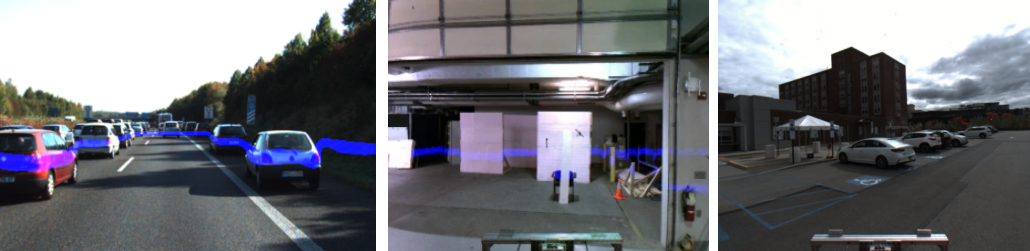
\includegraphics[width=1.0\textwidth]{figures/exp.png}
   \end{minipage}\hfill
   \centering
   \caption{Scenarios (a), (b), (c) from left to right}
   \label{fig:exp}
\end{figure}

\textbf{Planar Sweep:} A simple sanity check between simulation and the real sensor involves involves performing a uniform sweep across the scene in (b). 

\begin{figure}
   \centering
   \begin{minipage}{0.5\textwidth}
       \centering
       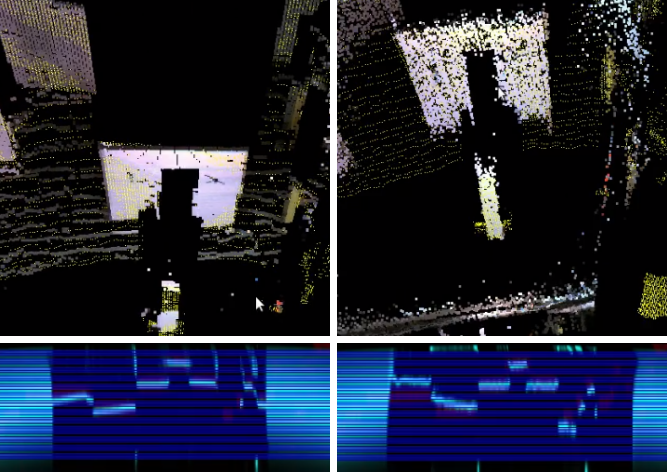
\includegraphics[width=1.0\textwidth]{figures/sweep.png}
   \end{minipage}\hfill
   \centering
   \caption{Doing a simple planar sweep across the scene. Colored pointcloud is the estimated depth, and Lidar ground truth in yellow. Left: LC simulated from the Lidar Depth. Right: Using the real LC}
   \label{fig:planarsweep}
\end{figure}

As seen in Fig. ~\ref{fig:planarsweep}, our simulated Light Curtain (LC) is able to reasonably match the real device. We also demonstrate how decreasing the steps the curtain takes reduces runtime but increases RMSE. Results seen in ~\ref{table:t1}

\begin{table}[h]
   \centering
   \begin{tabular}{|l|l|l|}
   \hline
    Policy&  Runtime/s&  RMSE/m\\ \hline
    Sweep 50 $\mathbf{C}$ Step 0.25m (Sim) &-  &1.156  \\ \hline
    Sweep 25 $\mathbf{C}$ Step 0.5m  (Sim) &-  &1.374  \\ \hline
    Sweep 50 $\mathbf{C}$ Step 0.25m (Real) &2  &1.284  \\ \hline
    Sweep 25 $\mathbf{C}$ Step 0.5m  (Real) &1  &1.574  \\ \hline
    Sweep 12 $\mathbf{C}$ Step 1.0m (Real) &0.5  &1.927  \\ \hline
   \end{tabular}
   \caption{Error wrt to time and number of Sweep steps}
   \label{table:t1}
\end{table}

Earlier, we had noted how $\sigma$ defined for each $C_{i}$ measurement in $P\left(\mathbf{c}_{t}|\mathbf{d}_{t}\right)$ is a function of the thickness of the curtain. We also experiment by making $\sigma$ fixed. We observe that $\sigma$ being a function of the curtain thickness is critical to better performance over larger steps/placements. Results seen in ~\ref{table:t2}

\begin{table}[h]
   \centering
   \begin{tabular}{|l|l|l|}
   \hline
    Policy&  Runtime/s&  RMSE/m\\ \hline
    Sweep $\mathbf{C}$ Step 0.25m (Dyn) &2  &1.276  \\ \hline
    Sweep $\mathbf{C}$ Step 0.5m  (Dyn) &1  &1.532  \\ \hline
    Sweep $\mathbf{C}$ Step 1.0m (Dyn) &0.5  &2.013  \\ \hline
    Sweep $\mathbf{C}$ Step 0.25m (Fixed) &2  &1.218  \\ \hline
    Sweep $\mathbf{C}$ Step 0.5m  (Fixed) &1  &1.658  \\ \hline
    Sweep $\mathbf{C}$ Step 1.0m (Fixed) &0.5  &2.290  \\ \hline
   \end{tabular}
   \caption{$\sigma$ in generated $P\left(\mathbf{c}_{t}|\mathbf{d}_{t}\right)$ being fixed vs being dynamic as a function of curtain thickness with real LC}
   \label{table:t2}
\end{table}

\textbf{Effect of Inverted Gaussian Model:} We attempt to run experiments on (a) and (b) testing the convergence time of policies $m0$ and $m1$, with $z=0.5$ and $z=1$ to test the effect of having 

% While this is a reasonable approach to estimating depth, it is also slow, as it requires placing many curtains. 

